\documentclass[12pt,letterpaper]{article}
\usepackage[utf8]{inputenc}
\usepackage[letterpaper, margin=1in]{geometry}
\usepackage{graphicx}
\graphicspath{{/}}

\title{MoNeT PYF Machine Learning}
\author{Ana Lucía Dueñas Chávez and Juan José Olivera Loyola \thanks{assisted by PhD. Benjamín Valdez (ITESM CQ) in collaboration with PhD. Héctor M. Sanchez (UCB)}}
\date{May 4, 2021}

\begin{document}
\maketitle
\begin{abstract}
In this report we explain the project objectives and steps performed to implement a lightweight ML tool
that approximates the results of a Mosquito population simulator.
\end{abstract}

\section{Introduction}
Mosquitos often carry diseases such as Dengue, Malaria, etc. That's why effort and economic investment
has been placed in researching management of species' populations via introduction of gentically modified
organisms who can surpress disease propagation. However, such actions require extensive knowledge
and obtaining it through real test and error experiments is both infeasable and dangerous.

MoNeT (Mosquito Networks Taskforce) was created to develop computer tools that are capable of simulating 
mosquito population dynamics, movement and genetics aiding biologists to solve for the right variables.
One of it's key reaseach lines is eliminating mosquitos in a population network of mosquitos in the
French Polynesia Island. MoNeT's simulator is capable of producing population dynamics outcomes.
However, it's computationally expensive, and during interdisciplinary meetings,
it's common to speculate on many possible configuration out of the air. A more lightweight tool is needed
to give immediate likely estimations for hypothesized configurations.

Machine Learning techniques have proven to be a general powerful tool for estimating functions and
statistical distrbution spaces given large amounts of sample data and training time. 
Besides being universal approximators, ML models take short computational time for making arbitrary estimations
and take very few memory space in comparison to the whole dataset they are approximating. 
Thus, ML techniques are a great technology to build
a quick estimation tool for experiment outcomes from prior data.
\section{Objective}
\subsubsection{Main Objective}
To produce a lightweight ML tool that can estimate elimination probability and time window results
of release experiments of genetically modified mosquitos.

\subsubsection{Subobjectives}
\begin{itemize}
    \item Interpretability: Understanding why a classification was made by the model is expected. Also, some confidence on the prediction is desireable.
    \item Framework Compliant: Prefereably built around scikit-learn. Has to accept numpy arrays and save and load models with joblib.
    \item Flexible Resolution: Model can be readjusted to a different dataset; same experiment but different zone of interest.
\end{itemize}

\section{Data Exploration}
\subsection{Features}
We begin by describing our dataset. Each experiment run is configured by 5 parameters:
\begin{itemize}
    \item (\emph{pop}) Population size per node % Entender bien esto porque lo maximo es 20, y 20 mosquitos suena a muy poco en ecosistema real
    \item (\emph{ren}) Number of weekly releases
    \item (\emph{res}) Release size % Que es fraccion de la poblacion estable? O sea originalmente
    % res es un numero entre [0,1]? La poblacion estable es la de pop? U otra poblacion, la de los mosquitos modificados en el lab?
    \item (\emph{mad}) Adult lifespan reduction % Este es un factor de proporcion dado por el gen, o es la cantidad de mosquitos esperados a reducir?
    \item (\emph{mat}) Male mating reduction    % Misma duda
\end{itemize}
So, we have a feature describing the environment where the mosquitos are to be released, 2 features describing a modification
on the mosquito organisms and finally 2 features to describe releasing modes.
\subsection{Target Variables}
MoNeT simulator outcomes can be analyzed with several metrics for each experiment configuration.
From these we try to predict two:
\begin{itemize}
    \item (\emph{POE}) Probability of Elimination
    \item (\emph{$WOP_{threshold}$}) Window of time that wild gene population is below a specific threshold.
\end{itemize}
Figure \ref{img:randomsimoutcomes}. shows several outcome instances by the simulator for the same configuration.
In the vertical axis we have the proportion of the population of mosquitos with the wild gene we are trying to surpress.
On the horizontal axis we have time in years. Each line represents a different outcome in the long run. 
We can observer for this configuration,
that all outcomes at first reduce significantly the target population the first year
, however, the population reestablishes in the following years for most of them.

\begin{figure}[h]
    \centering
    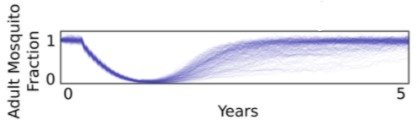
\includegraphics{randomsimoutcomes.jpg}
    \caption{Different possible outcomes for a single arbitrary experiment configuration.}
    \label{img:randomsimoutcomes}
\end{figure}

\subsection{Dataset Organization}
The dataset used for this project contains the results of 16,000 runs. However, each experiment run
has several random factors so it commonly generates mulitple outcomes as shown in Figure \ref{img:randomsimoutcomes}.
To account for this, simulation proportions are grouped by a worst case bound result and saved
under a file with the specific percentile associated (50\%, 75\%, 90\%). For example, let's say we 
read a Probability of Elimination Outcome ($POE_i$) of 0.83 for features $x_i$=$(pop=20, ren=8, res=10, mat=30, mad=20)$ for
the 50\% file. 
This means that 50\% of the simulations under this specific configuration resulted at least in a 70\% probability of elimination.
Then, if we were to see a \emph{POE} value of 0.71 for the same configuration on the 90\%, this would mean that configuration $x_i$,
most probable outcome bad, as the metric got lower when taking into account the majority of the simulation results.
Also, as more simulations are taking into consideration, the variance is expected to be lowest for percentil 50 and highest for percentil 90.

\subsection{Histograms}
We made a histogram of each feature to get a sense of the possible values they can take and their distribution.
\subsection{Correlations}
\subsection{Discretazing Target Variables}
\subsection{Understanding POE outcomes through decision trees}
\subsection{Understanding WOP outcomes throught 3D plotting}
%% Aqui van 5 histogramas, uno para cada variable
%  Podemos especular como podria afectar cada variable
%% Aqui va el histograma de POW y el de l




\section{Model Selection}
\subsection{Evaluating multiple configurations}
\subsection{Tree Results}
\subsection{KNN Results}
\subsection{NN Results}
\section{Pipeline Integration}
\section{Discussion}
\section{Conclusion}
\section{References}
\end{document}